\documentclass[11.5pt]{article}
\usepackage{stat110,float,enumitem}

\title{Continuous Random Variables}
\sectionnum{5}

\author{\justin, \michael, \creds}

%\SOLUTION

\begin{document}



\maketitle

\begin{notes}
\section*{Continuous Random Variables}

\begin{description}
\item[What is a Continuous Random Variable (CRV)?] A continuous random variable can take on any possible value within a certain interval (for example, [0, 1]), whereas a discrete random variable can only take on variables in a list of countable values (for example, all the integers, or the values 1, $\frac{1}{2}, \frac{1}{4}, \frac{1}{8}$, etc.)
\item[PMF's vs. PDF's] Discrete R.V's have Probability \textit{Mass} Functions, while continuous R.V.'s have Probability \textit{Density} Functions. We visualize a PDF as a graph where the $x$ axis is
\begin{center}
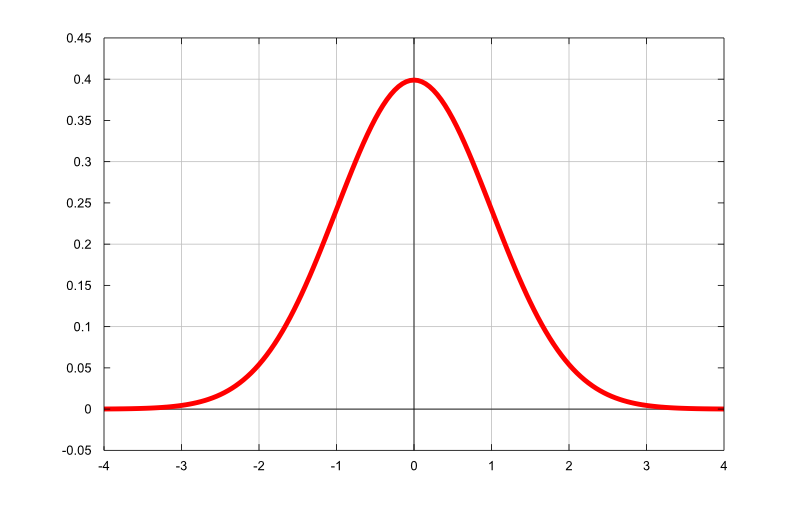
\includegraphics[scale=0.3]{normal_distribution.png}\\ 
\textbf{Normal PDF}
\end{center}

Intuitively, what do the $y$ values represent? Well it doesn't make sense to say $P(X = x)$ for a continuous r.v. $X$ because $P(X = x) = 0$ for all $x$. Think about the $y$ value in the above graph as: \textbf{the relative frequency for getting a value within $\epsilon$ of the $x$ value}
\item[What is the Cumulative Density Function (CDF)?] It is the following function of $x$.
		\[F(x) = P(X \leq x)\]
		With the following properties. 1) $F$ is increasing. 2) $F$ is right-continuous. 3) $F(x) \rightarrow 1$ as $x \rightarrow \infty$, $F(x) \rightarrow 0$ as $x \rightarrow -\infty$

\item[What is the Probability Density Function (PDF)?] The PDF, $f(x)$, is the derivative of the CDF. 
\[ F'(x) = f(x) \]
Or alternatively,
\[ F(x) = \int_{-\infty}^x f(t)dt \]
Note that by the fundamental theorem of calculus,
\[ F(b) - F(a) = \int^b_a f(x)dx \]
Thus to find the probability that a CRV takes on a value in an interval, you can integrate the PDF, thus finding the area under the density curve.

Two additional properties of a PDF:  it must integrate to 1 (because the probability that a CRV falls in the interval $[-\infty, \infty]$ is 1, and the PDF must always be nonnegative.
\[\int^\infty_{-\infty}f(x)dx \hspace{2 cm} f(x) \geq 0\]
\item[How do I find the expected value of a CRV?] Where in discrete cases you sum over the probabilities, in continuous cases you integrate over the densities.
\[E(X) = \int^\infty_{-\infty}xf(x)dx \]
Review: Expected value is \emph{linear}. This means that for \emph{any} random variables $X$ and $Y$ and any constants $a, b, c$, the following is true:
\[E(aX + bY + c) = aE(X) + bE(Y) + c\]
\end{description}

\section*{Discrete versus Continuous}
\begin{table}[htb!] \begin{center}
	\begin{tabular}{ccc}
	\toprule
		~ & \textbf{Discrete} & \textbf{Continuous} \\ \midrule
		$P(X \leq x) = $  & $F(x)$ (CDF) & $F(x)$ (CDF) \\ 
		To find probabilities, & Add over PMF $P(X = x)$ & Integrate over PDF $f(x) = F'(x)$ \\ 
		$E(X) =$ & $\sum_x xP(X=x)$ & $\int_{-\infty}^{\infty}xf(x)dx$ \\ 
		$E(g(X)) =$ & $\sum_x g(x)P(X=x)$ (LOTUS Discrete) & $\int_{-\infty}^{\infty} g(x)f(x)dx$ (LOTUS Continuous)
	\end{tabular}\end{center}
\end{table}


\section*{Variance}
\begin{description}
\item[What is Variance?] Variance is the expected squared distance away from the mean. It is the square of the standard deviation.
\[\var(X) = E((X - EX)^2) = E(X^2) - E(X) \]
Oftentimes it's easier to calculate $E(X^2) - E(X)$ rather than $E(X - EX)$. You can find $E(X^2)$ with LotUS.

%The following is true for constants $a, b$:
\[\var(aX + b) = a^2\var(X)\]
The following is true \textbf{only if X and Y are independent}:
\[\var(X + Y) = \var(X) + \var(Y)\]
\end{description}


\section*{Universality of Uniform} When you plug any random variable into its own CDF, you get a Uniform[0,1] random variable. When you put a Uniform[0,1] into an inverse CDF, you get the corresponding random variable. For example, let's say that a random variable X has a CDF
	\[ F(x) = 1 - e^{-x} \]
	By the Universality of the the Uniform, if we plug in X into this function then we get a uniformly distributed random variable.
	\[ F(X) = 1 - e^{-X} \sim U\]
	Similarly, since $F(X) \sim U$ then $X \sim F^{-1}(U)$. The key point is that \emph{for any continuous random variable X, we can transform it into a uniform random variable and back by using its CDF.}
\begin{center} 
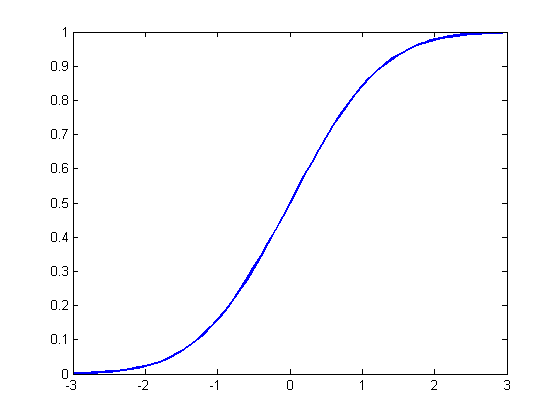
\includegraphics[scale = 0.5]{normal_cdf.png}\\
\textbf{Normal CDF}
\end{center}
In the CDF of the Normal(0,1) distribution above, if we choose a number between 0 and 1 uniformly at random on the $y$ axis, we see that the distribution of $x$ values is normal. 
\section*{Uniform Distribution (Continuous)}
\begin{description}
\item Let us say that $U$ is distributed $\Unif(a, b)$. We know the following:
\begin{description}
	\item[Properties of the Uniform] For a uniform distribution, the probability of an draw from any interval on the uniform is proportion to the length of the uniform. The PDF of a Uniform is just a constant, so when you integrate over the PDF, you will get an area proportional to the length of the interval.
	\item[PDF and CDF] 
\begin{eqnarray*}
\Unif(a, b)
  \hspace{.65 in}
   f(x) = \left\{
     \begin{array}{lr}
       \frac{1}{b-a} & x \in [a, b] \\
       0 &  x \notin [a, b]
     \end{array}
   \right.
   \hspace{.75 in}
   F(x) = \left\{
     \begin{array}{lr}
       0 & x < a \\
       \frac{x-a}{b-a} & x \in [a, b] \\
       1 &  x > b
     \end{array}
   \right. 
\end{eqnarray*}


	
\end{description}
\end{description}

\section*{Normal Distribution (Continuous) (aka Gaussian)}
\begin{description}

\item Let us say that $X$ is distributed $\N(\mu, \sigma^2)$. We know the following:
\begin{description}
	\item[Central Limit Theorem] The Normal distribution is ubiquitous because of the central limit theorem, which states that averages of independent identically-distributed variables will approach a normal distribution regardless of the initial distribution.
	\item[Transformable] Every time we stretch or scale the normal distribution, we change it to another normal distribution. If we add $c$ to a normally distributed random variable, then its mean increases additively by $c$. If we multiply a normally distributed random variable by $c$, then its variance increases multiplicatively by $c^2$. Note that for every normally distributed random variable $X \sim \N(\mu, \sigma^2)$, we can transform it to the standard $\N(0, 1)$ by the following transformation:
	\[\frac{X - \mu}{\sigma} \sim \N(0, 1) \]
	\item[Example] Heights are normal. Measurement error is normal. By the central limit theorem, the sampling average from a population is also normal.
	\item[Standard Normal] - The Standard Normal, denoted $Z$, is $Z \sim \N(0, 1)$
	\item[PDF]
\[ f(x)=\frac{1}{\sigma \sqrt{2\pi}} e^{-\frac{(x - \mu)^2}{2 \sigma^2}} \]
	\item[CDF] - It's too difficult to write this one out, so we express it as the function $\Phi(x)$
\end{description}
\end{description}

\section*{Continuous Distributions}
\begin{center}
\renewcommand{\arraystretch}{3}
\begin{tabular}{cccccc}
\textbf{Distribution} & \textbf{PDF and Support} & \textbf{Expected Value}  & \textbf{Variance} \\
\hline

\shortstack{Uniform \\ \Unif($a, b$)} & \shortstack{$ f(x) = \frac{1}{b-a}, x \in [a, b] $ \\$ f(x) = 0, x \notin [a, b]$} & $\frac{a+b}{2}$ & $\frac{(b-a)^2}{12}$  \\
\hline
\shortstack{Normal \\ $\N(\mu, \sigma^2)$} & $f(x) = \frac{1}{\sigma \sqrt{2\pi}} e^{-\frac{(x - \mu)^2}{2 \sigma^2}}$ & $\mu$  & $\sigma^2$  \\
\hline
\shortstack{Exponential \\ $\Expo(\lambda)$} & \shortstack{$f(x) = \lambda e^{-\lambda y}, x \in [0, \infty)$\\$ f(x) = 0, x \notin [0, \infty)$} & $\sfrac{1}{\lambda}$ & $\sfrac{1}{\lambda^2}$\\
\hline

\end{tabular}
\end{center}

\section*{Exponential Distribution (Continuous)}

Let us say that $X$ is distributed $\Expo(\lambda)$. We know the following:
\begin{description}
	\item[Story] You're sitting on an open meadow right before the break of dawn, wishing that airplanes in the night sky were shooting stars, because you could really use a wish right now. You know that shooting stars come on average every 15 minutes, but it's never true that a shooting star is ever "due" to come because you've waited so long. Your waiting time is memorylessness, which means that the time until the next shooting star comes does not depend on how long you've waited already.
	
	\item[Example] The waiting time until the next shooting star is distributed $\Expo(4)$. The 4 here is $\lambda$, or the rate parameter, or how many shooting stars we expect to see in a unit of time. The expected time until the next shooting star is $\frac{1}{\lambda}$, or $\frac{1}{4}$ of an hour. You can expect to wait 15 minutes until the next shooting star.
	
	\item[All Exponentials are Scaled Versions of Each Other]
		\[Y \sim \Expo(\lambda) \rightarrow X = \lambda Y \sim \Expo(1)\]
	 
	\item[PDF and CDF] The PDF and CDF of a Exponential is:
\begin{eqnarray*}
f(x) = \lambda e^{-\lambda x},
\hspace{.1 in}
x \in [0, \infty)
\hspace{1 in}
F(x) = P(X \leq x) = 1 - e^{-\lambda x},
\hspace{.1 in}
x \in [0, \infty)
\end{eqnarray*}
	

	\item[Memorylessness] The Exponential Distribution is the sole continuous memoryless distribution. This means that it's always ``as good as new", which means that the probability of it failing in the next infinitesimal time period is the same as any infinitesimal time period. This means that for an exponentially distributed $X$ and any real numbers $t$ and $s$,
	\[P(X > s + t | X > s) = P(X > t)\]
	Given that you've waited already at least $s$ minutes, the probability of having to wait an additional $t$ minutes is the same as the probability that you have to wait more than $t$ minutes to begin with. Here's another formulation.
	\[X - a | X > a \sim \Expo(\lambda)\]


\end{description}

\end{notes}
\newpage 
\section*{Practice Problems}

\begin{exercise}{Birthdays}
Use Poisson approximations to investigate the following types of coincidences. The usual assumptions of the birthday problem apply, such as that there are 365 days in a year, with all days equally likely.
\begin{enumerate} [(a)]
\item How many people are needed to have a 50\% chance that at least one of them has the same birthday as \textit{you}?
\item How many people are needed to have a 50\% chance that there are two people who not only were born on the same day, but also were born at the same hour (e.g., two people born between 2 pm and 3 pm are considered to have been born at the same hour).
\end{enumerate}
\end{exercise}

\begin{solution}{3}
\begin{enumerate}[(a)]
\vspace{-1em}
\item Let $k$ be the number of people there are other than you. Create an indicator variable $I_i$ for each of the $k$ people as to whether they have the same birthday as you. Then, $P(I_i = 1) = \frac{1}{365}$ and thus $E\left[ \sum_{i = 1}^{k} I_i \right] = \frac{k}{365}$. Therefore, we can model this as a $\text{Pois} \left( \frac{k}{365} \right)$ and so we just need to calculate 
$$ 1 - e^{-k/365} = 0.5$$ 
It turns out that $k \approx 253$. 
\item This is the birthday problem but with $365 \cdot 24$ types instead of just 365. Creating an indicator r.v. for whether each pair of $k$ people have the same birthday, we get that the number of pairs of people with the same birthday is distributed approximately $\text{Pois} \left( \frac{{k \choose 2}}{365 \cdot 24}  \right)$ and thus the probability of at least people having the same birthday is approximately: 
$$ 1 - e^{-\frac{{k \choose 2}}{365 \cdot 24}}$$
Setting it equal to $\frac{1}{2}$ gives us $k = 111$. 

\end{enumerate}
\end{solution}


\begin{exercise}{Uniform Power} 
Let $U \sim \Unif(-1,1)$
\begin{enumerate}
\item Compute $E(U), \var(U), E(U^4)$. 

\item Find the PDF and CDF of $U^2$. Is it also a uniform distribution? 
\end{enumerate}
\end{exercise}
\begin{solution}{3} 
When trying to compute the PDF of a transformation, we usually work from the CDF first. Note that the PDF of $U$ is $f(x) = \frac{1}{2}$. 
\begin{enumerate}
\item $E(U) = 0$ because the distribution is symmetric about 0. We need to calculate $E(U^2)$ for the variance, so we have:

$$ E(U^2) = \int_{-1}^{1} u^2 \cdot \frac{1}{2} \diff u = \left[\frac{1}{6} u^3\right]_{-1}^{1} = \frac{1}{3}$$ 
Therefore, $\var\paren{U} = E(U^2) - E(U)^2 = \boxed{\frac{1}{3}}$ 

Next, we do the same for $E(U^4)$: 

$$ E(U^4) = \int_{-1}^{1} u^4 \cdot \frac{1}{2} \diff u = \left[\frac{1}{10} u^5\right]_{-1}^{1} = \boxed{\frac{1}{5}}$$

\item We first find the CDF. $$P(U^2 < k) = P(-\sqrt{k} < U < \sqrt{k}) = \frac{2\sqrt{k}}{2} = \sqrt{k}$$, which we can easily calculate graphically. If this wasn't possible to do graphically, then we would integrate the PDF of $U$ between $-k$ and $k$. 

Therefore, the PDF is: 

$$ \frac{d}{dk} P(U^2 < k) = \boxed{\frac{1}{2 \sqrt{k}}}$$

This is definitely \textbf{not} a uniform distribution. This also shows that $U^k$ is not uniform anymore for any $k > 1$.
\end{enumerate}
\end{solution}

 \begin{exercise}{Normal Squared}
 Let $Z \sim N(0,1)$ with CDF $\Phi$. The PDF of $Z^2$ is the function given by: 

 $$ g(w) = \frac{1}{\sqrt{2\pi w}} e^{-w/2}$$ with a support of $w \geq 0$. 

 \begin{enumerate}[(a)]
 \item Find expressions for $E(Z^4)$ as integrals in two different ways, one based on the PDF of $Z$ and the other based on the PDF of $Z^2$. 

 \item Find $E(Z^2 + Z + \Phi(Z))$. 

 \item Find the CDF of $Z^2$ in terms of $\Phi$; do not find the PDF of $g$. 
 \end{enumerate}

 \end{exercise}

 \begin{solution}{3}
 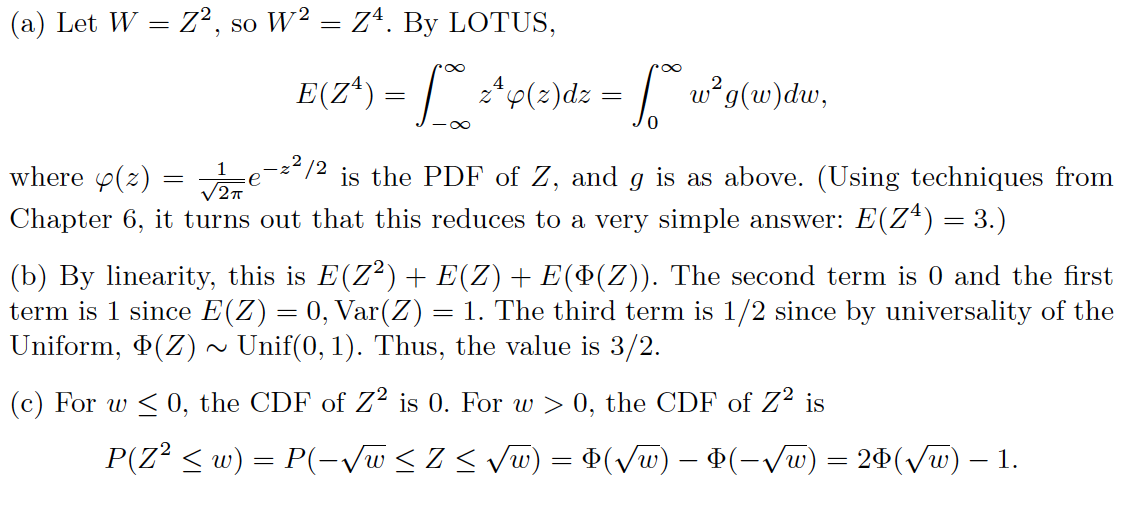
\includegraphics[scale=0.7]{normal_sol.png}
 \end{solution}

\begin{exercise}{Breaking Sticks}
A stick of length 1 is broken at a uniformly random point yielding two pieces. Let $X$ and $Y$ be the lengths of the shorter and longer pieces, respectively, and let $R = \frac{X}{Y}$ be the ratio of the lengths $X$ and $Y$. 
\begin{enumerate} [(a)]
\item Find the CDF and PDF of $R$
\item Find the expected value of $R$ (if it exists). 
\end{enumerate}

\begin{solution}{3} 
\begin{enumerate}
\item Let $U \sim \Unif(0,1)$ represent the location of the break, and let $X = \min(U, 1-U)$. As a side note, recall that $U$ and $1-U$ have the same distribution of $\Unif(0,1)$. For some value $r \in (0,1)$, we have that 
    $$P(R \leq r) = P(\frac{X}{Y} \leq r) = 
    P(X \leq r (1-X)) = P (X \leq \frac{r}{1+r})$$
However, to fully evaluate this, we must find the CDF of $X$. To do so, we first recognize that, because $X$ is the minimum of two random variables, it is easier to consider the event $\{X > x\}$, as this event is equivalent to saying $\{U > x, 1-U > x\}$ (if the minimum of two values is greater than $x$, then the other must also be greater than $x$). We thus have that
    $$P(X \leq x) = 1 - P(X > x) = 1-P(U > x, 1-U >x) = 1 -
    P(x < U < 1-x) = 2x$$
Therefore, we have that the CDF of $R$ is simply
    $$P(R \leq r) = \frac{2r}{1+r}$$
To find the PDF we differentiate with respect to $r$ and find that 
    $$f_R(r) = \frac{2}{(1+r)^2}$$
\item Letting $t = 1+r$, we have 
    $$E(R) = 2 \int_0^1 \frac{r}{(1+r)^2} dr = 2 \int_1^2 
    \frac{t-1}{t^2} dt = 2\int_1^2 \frac{1}{t} dt - 2 
    \int_1^2 \frac{1}{t^2} dt = 2 \ln 2 - 1$$
\end{enumerate}
\end{solution}
\end{exercise}

\begin{exercise}{Universality of the Uniform} 
 Let $U \sim \Unif(0,1)$, and let $X = -(\log(1-U))^{1/3}$. Find the CDF and PDF of $X$.
\end{exercise}

\begin{solution}{0.5} 
We calculate $P(x \leq X)$, but use the substitution given to try and solve a Uniform distribution's CDF instead: 

\begin{align*}
P(X \leq x) &= P(-(\log(1-U))^{1/3} \leq x)\\
 & = P(\log(1-U)^{1/3}) \geq -x) \\ 
&= P(\log(1-U) \geq -x^3)  \\ 
&= P(1 - e^{-x^3} \geq U) \\
&= P(U \leq 1 - e^{-x^3})\\
&= \boxed{(1 - e^{-x^3})}
\end{align*}
which is the CDF of $X$. 

The PDF of $x$ is the derivative, so: $$ f(x) = \pder[]{x} (1 - e^{-x^3}) = 3x^2 e^{-x^3}$$

\end{solution}

% \begin{exercise}{HUHS}
% There are $n$ couples, each of which has exactly 1 child.  There is a mix-up at the hospital, and they distribute the $n$ children randomly among the $n$ couples.  Let $X$ be the number of couples that get their baby back.
% \begin{enumerate}
%     \item As a refresher, find $E(X)$.
%     \item What is the probability that no one gets their baby back as $n\to\infty$?
% \end{enumerate}
% \end{exercise}
% \begin{solution}{0.5}
% \begin{enumerate}
%     \item Define $n$ indicators $I_j$ where the indicator represents the $j$-th couple getting their own child back. The expected value of every indicator is \[E(I_j)=\frac{1}{n}\] and we have $n$ total indicators, so by linearity of expectation, \[E(X) = \frac{1}{n}\cdot n = 1\]
%     \item The probability that no one gets their baby back is given by $P(X=0)$. Since we have many (loosely) independent events, each with a small probability of success, we can use the Poisson paradigm. Our $\lambda$ is just the sum of all the individual probabilities, which is $n\cdot \frac{1}{n}=1$, as we showed above. \\ So we approximately have $X\backsim \Pois(1)$. Knowing the PMF of a Poisson, we can now just plug $X=0$ back into the PMF and get \[P(X=0) = e^{-1}\]
% \end{enumerate}
% \end{solution}



 \begin{exercise}{Finishing Homework} 
 Three students are working independently on their probability homework. All 3 start at 1 pm on a certain day, and each takes an Exponential time with mean 6 hours to complete the homework. What is the earliest time when all 3 students will have completed the homework, on average?  (That is, at this time all 3 students need to be done with the homework.)
 \end{exercise}

\begin{solution}{3} 
 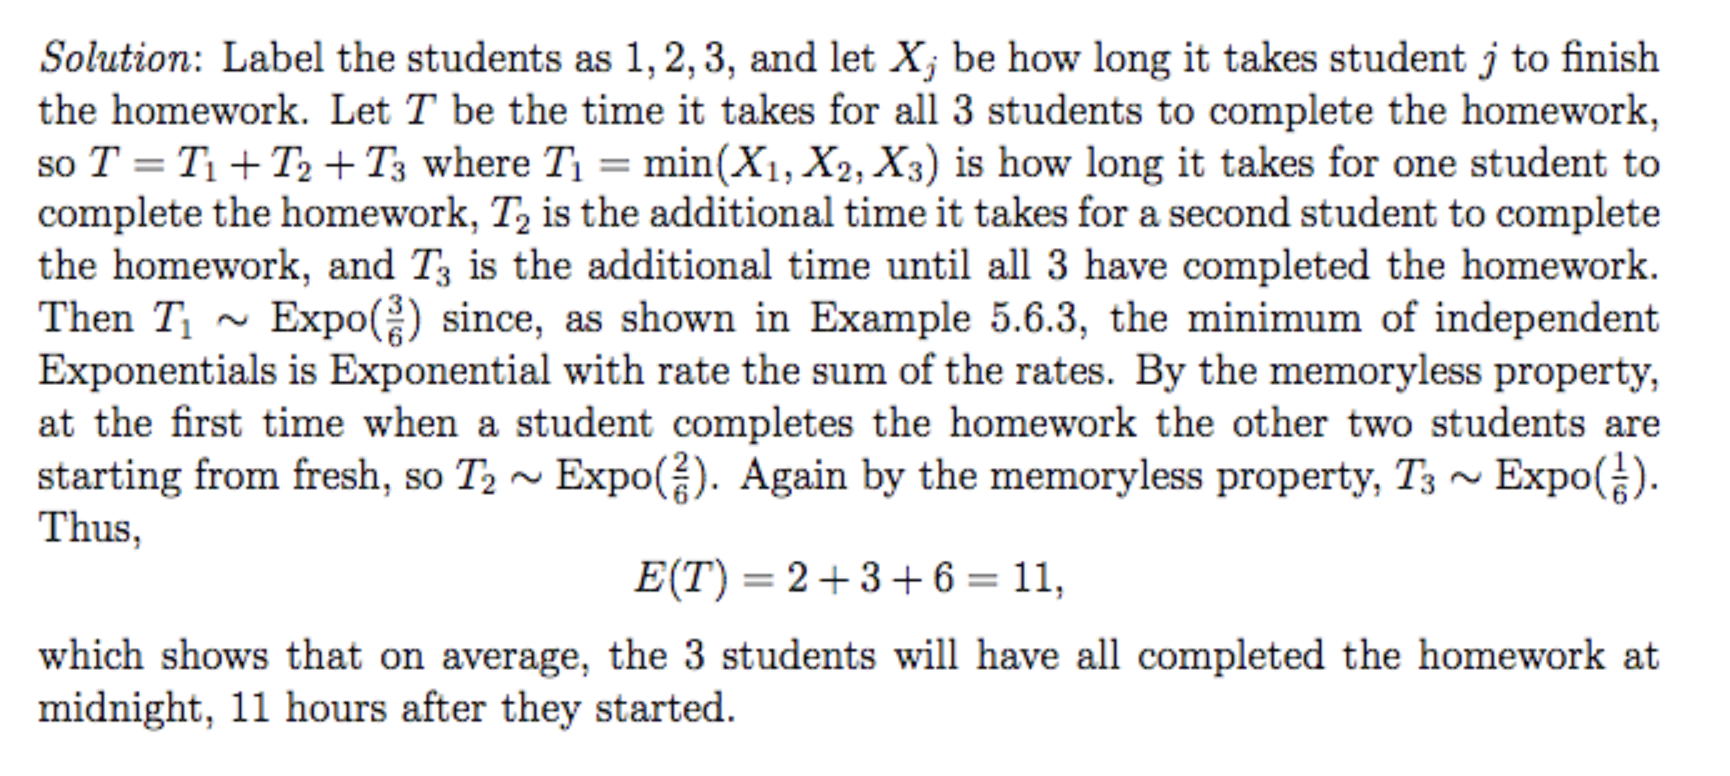
\includegraphics[width=16cm]{expo_hw_sol.png}
 \end{solution} 

\begin{exercise}{Continuous RV manipulation}
Let $X$ be a continuous r.v. with CDF $F$ and PDF $f$.
\begin{enumerate}
    \item Find the conditional CDF $X$ given that $X>a$ (where $a$ is a constant with $P(X>a)\neq0$).
    \item Find the conditional PDF of $X$ given $X > a$ (this is the derivative of the conditional CDF).
    \item Check that the conditional PDF from (b) is a valid PDF, by showing directly that it is nonnegative and integrates to 1.
\end{enumerate}
\end{exercise}
\begin{solution}{2}
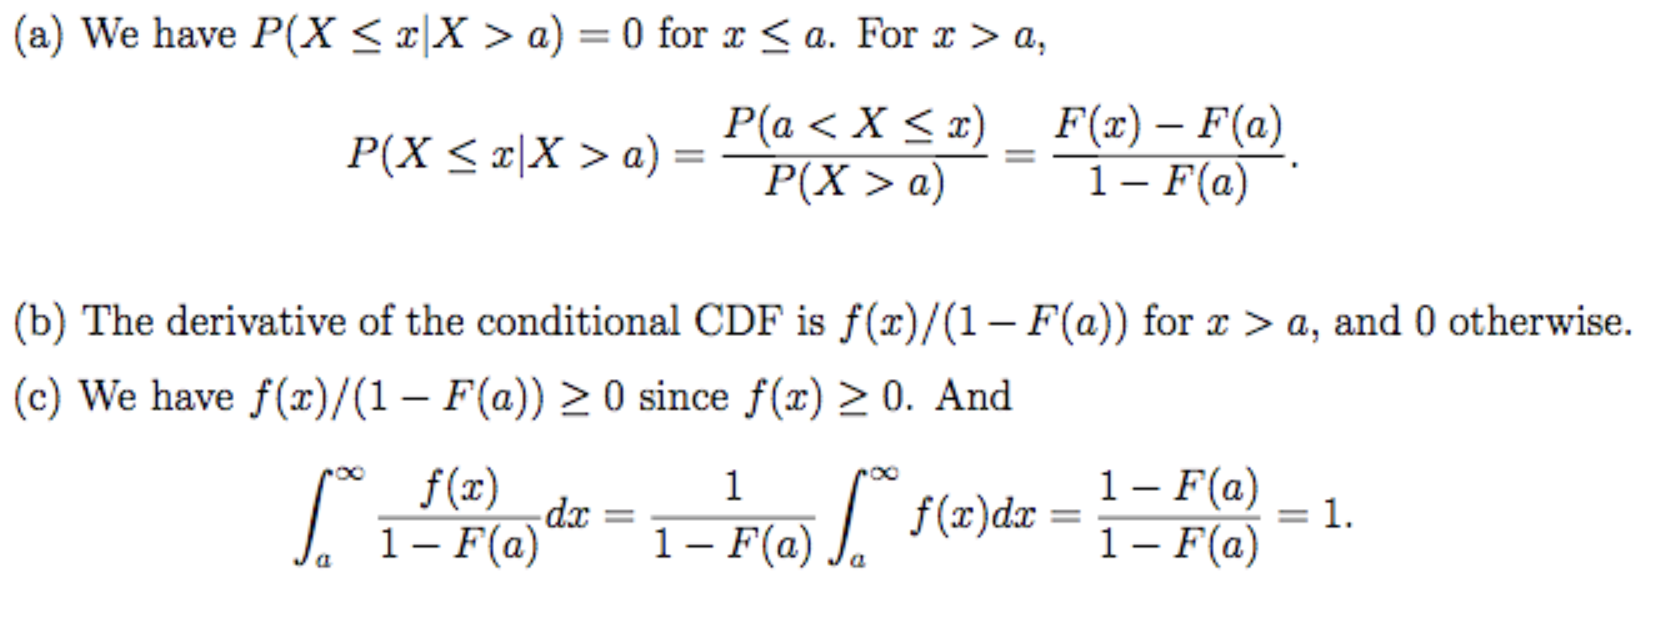
\includegraphics[width=16cm]{generalrv_sol.png}
\end{solution}

% \begin{exercise}{CDF} 
% Let $F(x) = e^{-e^{-x}}$. This is the CDF of a random variable of what is known as the Gumbel distribution. Note that $F(x)$ It is continuous and strictly increasing. Let $X$ have CDF $F$ and let $W = F(X)$. Find the mean and variance of $W$.
% \end{exercise} 

% \begin{solution}{0.5}
% We notice that $X$ has CDF $F(x)$, yet we are transforming $X$ by its own CDF. Universality of the Uniform tell us that plugging a continuous random variable into its own CDF results in the uniform distribution because there is a 1-1 correspondence between $\Unif(0,1)$ and $X$, a function which takes $x$ in the support of $X$ and maps it to $CDF(x)$. Therefore, $F(X) \sim \Unif(0,1)$, so the mean is $\frac{1}{2}$ and the variance is $\frac{1}{12}$ just like in the uniform. 
% \end{solution}

% \section*{Additional Problems}

% \begin{exercise}{Survey} 
% A survey is being conducted in a city with a million ($10^6$) people. A sample of size 1000 is collected by choosing people in the city at random, with replacement and with equal probabilities for everyone in the city. Find a simple, accurate approximation to the probability that at least one person will get chosen more than once. 
% \end{exercise}

% \begin{solution}{0.5} 
% Let $I_{ij}$ be the the indicator that the $i$th and $j$th sampled people will be the same person and let $X$ b the sum of the $I_{ij}$'s. We are interested in approximating $P(X \geq 1)$, which is the probability that at least one of the $I_{ij}$'s is equal to 1. There are ${1000 \choose 2}$ $X_{ij}$'s, each of which has probability $\frac{1}{10^6}$ of happening. Therefore, the expectation is: 

% $$ E(X) = {1000 \choose 2} \frac{1}{10^6} = \frac{1000 \cdot 999}{2 \cdot 10^6} \approx \frac{1}{2}$$ 

% Now, we know that on average, $1/2$ out of the ${1000 \choose 2}$ combinations of two surveyed people, will be of the same person. Since there are lots ${1000 \choose 2}$ of possible ways for two surveys to survey the same person, but the probability of each pair of surveys surveying the same person is small ($1/10^6$) and seemingly independent, we can approximate the distribution of pairs of same-responders with a Pois(1/2) distribution. $X \sim \Pois(1/2)$ and we are interested in $P(X > 0)$ which would be $$ 1 - P(X = 0) = \boxed{1 - e^{-1/2}}$$
% \end{solution}

\begin{exercise}{Pareto Distribution} 
The Pareto distribution with parameter $a > 0$ has PDF $f(x) =\frac {a}{x^{a+1}}$ for $x \geq 1$ (and 0 otherwise). This distribution is often used in statistical modeling. 
\begin{enumerate}
\item Find the CDF of a Pareto r.v. with parameter $a$; check that it is a valid CDF. 

\item Suppose that for a simulation you want to run, you need to generate i.i.d. Pareto(a) r.v.s. You have a computer that knows how to generate i.i.d. $\Unif(0, 1)$ r.v.s but does not know how to generate Pareto r.v.s. Show how to do this.
\end{enumerate}

\end{exercise}

\begin{solution}{3}
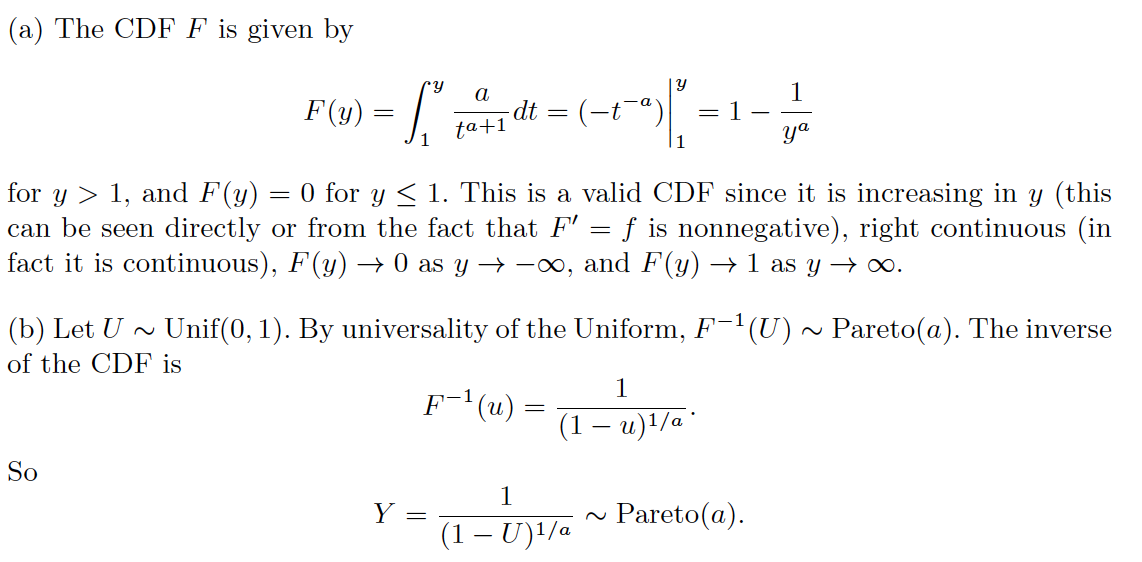
\includegraphics[scale=0.7]{pareto_sol.png}

\end{solution}

\end{document}
